% Copyright 2008 by Christian Feuersaenger
%
% This file may be distributed and/or modified
%
% 1. under the LaTeX Project Public License and/or
% 2. under the GNU Free Documentation License.
%
% See the file doc/generic/pgf/licenses/LICENSE for more details.
\section{Externalization Library}
\label{section-libs-external}
{\noindent {\emph{by Christian Feuers\"anger}}}

\begin{tikzlibrary}{external}
	This library provides a high-level automatic or semi--automatic export feature for \tikzname\ pictures.
	Its purpose is to convert each picture to a separate \pdf.
\end{tikzlibrary}

\subsection{Overview}

There are several reasons why external images for at least some pictures are of interest:
\begin{enumerate}
	\item Larger picture require a considerable amount of time, which is necessary for every compilation. However, only few images will change from run to run. It can simply save time to export finished images and include them as final graphics.
	\item It may be desirable to have final images for some graphics, for example to include them in third-party programs or to communicate them electronically.
	\item It may be necessary to typeset a file in environments where \pgfname\ and \tikzname\ are not available. In this case, external images are the only way to ensure compatibility.
\end{enumerate}
The purpose of this library is to provide a way to export any \tikzname-picture to separate \pdf\ (or \eps) images without changing the main document. It employs the |\beginpgfgraphicnamed| $\dotsc$ |\endpgfgraphicnamed| framework of \pgfname\ which is discussed in section~\ref{section-external}.

\subsection{Requirements}
For most users, the library does not need special attention since requirements are met anyway. It collects all tokens between |\begin{tikzpicture}| and the next following |\end{tikzpicture}| and replaces them by the appropriate graphics or it takes steps to generate such an image.% For Con\TeX t and plain \TeX\ users, the appropriate begin and end picture statements apply.

It can't expand macros during this step, so the only requirement is that every picture's end is directly reachable from its beginning, without further macro expansion. Furthermore, the library assumes that all \LaTeX\ pictures are ended with |\end{tikzpicture}|.% In Con\TeX t, the end command is assumed to be |\stoptikzpicture| and for plain \TeX\ it is |\endtikzpicture|.

The library always searches for the \emph{next} picture's end, |\end{tikzpicture}|. As a consequence, you can't use nested pictures directly. You \emph{can} nest pictures, but you have to avoid that the nested picture's |\end| command is found before the outer |\end| command (for example using bracing constructs or by writing the nested picture into a separate macro call).

\subsection{A word about Con\TeX t and plain \TeX}
Currently, the basic layer backend |\beginpgfgraphicnamed| $\dotsc$ |\endpgfgraphicnamed| relies on \LaTeX\ only, so externalization is only supported for \LaTeX\ yet.
%The library comes in three different versions, one for \LaTeX, one for Con\TeX t and one for plain \TeX. For reasons of simplicity, examples in this manual only refer to \LaTeX\ (especially |pdflatex|).

\subsection{Externalizing graphics}
After loading the library, a call to |\tikzexternalize| is necessary to activate the externalization.
\begin{codeexample}[code only]
\documentclass{article}
% main document, called main.tex
\usepackage{tikz}

\usetikzlibrary{external}
\tikzexternalize{main} % provide the file's real name

\begin{document}
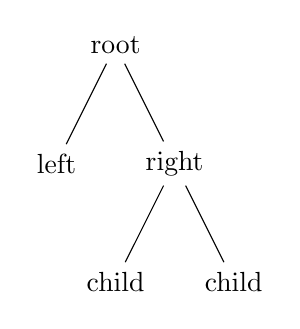
\begin{tikzpicture}
  \node {root}
    child {node {left}}
    child {node {right}
      child {node {child}}
      child {node {child}}
    };
\end{tikzpicture}

A simple image is \tikz \fill (0,0) circle(5pt);.
\end{document}
\end{codeexample}
It is necessary to configure the file's name, in our case |main.tex|.

The method works as follows: if the document is typeset normally, the library searches for replacement images for every picture. Filenames are generated automatically if there is no explicit file name. In our case, the two file names will be |main-figure0| and |main-figure1|. If they exist, those images are simply included and the pictures as such are not processed. If graphics file do not exists, steps are taken to generate the missing ones. 
Missing images need to be generated by a separate run of \LaTeX\ in which the |\jobname| is set to the desired image file name.
\begin{codeexample}[code only]
pdflatex -jobname main-figure0 main
pdflatex -jobname main-figure1 main
\end{codeexample}
In the default configuration |mode=convert with system call|, these commands are issued automatically by using the |\write18| method to call system commands. It is also possible to output every required file name; users will need to issue these command manually (or with a script). The probably most comfortable way is to use the default configuration with
\begin{codeexample}[code only]
pdflatex -shell-escape main
\end{codeexample}
\noindent which automatically calls |pdflatex -jobname |\marg{image} \marg{main}.

If the library realizes that the jobname differs from the argument of |\tikzexternalize|, it enters its conversion mode. During the evaluation of
\begin{codeexample}[code only]
pdflatex -jobname main-figure0 main
\end{codeexample}
\noindent \pgfname\ changes the shipout routine. The complete file |main.tex| is typeset as normal, but only the part of the desired picture will be written to the output file, in our case |main-figure0.pdf|. The rest of the document is silently thrown away. Of course, such a conversion process is quite expensive since we need to do it for every picture. Since everything except the current picture is thrown away, the library skips all other pictures. Furthermore, any |\includegraphics| commands which are outside of the converted \tikzname-picture will be skipped as well. Thus, the conversion process should be much faster than typesetting the complete document, but it still requires its time.

Finally, all images will be converted. From this point on, successive runs of \LaTeX\ will use the final graphics files, the pictures won't be used anymore. Section~\ref{section-libs-external-nopgf} contains details about how to submit such a file to environments where \pgfname\ is not available.

\begin{command}{\tikzexternalize[\meta{optional arguments}]\marg{real file name}}
	This command activates the externalization. It installs commands to replace every \tikzname-picture. It needs to be called before |\begin{document}| because it may need to install its separate shipout routine.

	The argument \marg{real file name} denotes the file's name, without the |.tex| extension. It is used to generate picture filenames (by appending |-figure|\marg{number}) and to decide whether a new shipout routine needs to be installed (if |\jobname| has a different value).

	The \meta{optional argument} can be any of the keys described below.
\end{command}

\begin{key}{/tikz/external/system call=\marg{template}}
\label{extlib:systemcall:option}
	A template string used to generate system calls. Inside of \marg{template}, the macro |\image| can be used as placeholder for the image which is about to be generated while |\texsource| contains the main file name.

	The default is 
\begin{codeexample}[code only]
\tikzset{external/system call={pdflatex -shell-escape -halt-on-error 
    -interaction=batchmode -jobname "\image" "\texsource"}
\end{codeexample}

	For |eps| output, you can (and need to) use
\begin{codeexample}[code only]
\tikzset{external/system call={latex -shell-escape -halt-on-error
    -interaction=batchmode -jobname "\image" "\texsource"; 
    dvips -o "\image".ps "\image".dvi}}
\end{codeexample}
	
	The argument \marg{template} will be expanded using |\edef|, so any control sequences will be expanded. During this evaluation, `|\\|' will result in a normal backslash, `|\|'. Furthermore, double quotes `|"|', single quotes `|'|', semicolons and dashes `|-|' will be made to normal characters if any package uses them as macros. This ensures compatibility with the |german| package, for example.
\end{key}

\subsubsection{Customizing the Generated File Names}
The default filename for externalized graphics is `\meta{real file name}|-figure_|\meta{number}' where \meta{number} ranges from $0$ to whatever is required. However, there are a couple of ways to change the generated filenames:
\begin{itemize}
	\item Changing the overall file name using a |prefix|,
	\item Changing the file name for a single figure using |\tikzsetnextfilename|,
	\item Changing the file name for a restricted set of figures using |figure name|.
\end{itemize}

\begin{key}{/tikz/external/prefix=\marg{file name prefix} (initially empty)}
	A shortcut for |\tikzsetexternalprefix|\marg{file name prefix}.
\end{key}

\begin{command}{\tikzsetexternalprefix\marg{file name prefix}}
	Assigns a common prefix used by all file names. For example,
\begin{codeexample}[code only]
\tikzsetexternalprefix{figures/}
\end{codeexample}
	will prepend |figure/| to every external graphics file name.

	Please note that |\tikzsetexternalprefix| is the \emph{only} way to assign a prefix in case you want to prepare your document for environments where \pgfname\ is not installed (see section~\ref{section-libs-external-nopgf}).
\end{command}

\begin{command}{\tikzsetnextfilename\marg{file name}}
	Sets the file name for the \emph{next} \tikzname\ picture or |\tikz| short command. It will \emph{only} be used for the next picture.

	Pictures for which no explicit file name has been set will get automatically generated file names.

	Please note that |prefix| will still be prepended to \marg{file name}.
\begin{codeexample}[code only]
\documentclass{article}
% main document, called main.tex
\usepackage{tikz}

\usetikzlibrary{external}
\tikzexternalize[prefix=figures/]{main} % provide the file's real name

\begin{document}

\tikzsetnextfilename{trees}
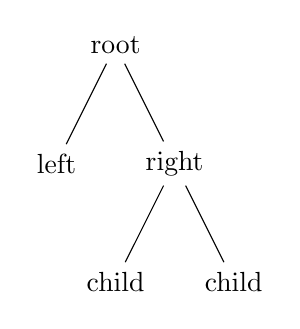
\begin{tikzpicture} % will be written to 'figures/trees.pdf'
  \node {root}
    child {node {left}}
    child {node {right}
      child {node {child}}
      child {node {child}}
    };
\end{tikzpicture}

\tikzsetnextfilename{simple}
A simple image is \tikz \fill (0,0) circle(5pt);. % will be written to 'figures/simple.pdf'


\begin{tikzpicture} % will be written to 'figures/main-figure0.pdf'
   \draw[help lines] (0,0) grid (5,5);
\end{tikzpicture}
\end{document}
\end{codeexample}
\begin{codeexample}[code only]
pdflatex -shell-escape main
\end{codeexample}
\end{command}

\begin{key}{/tikz/external/figure name=\marg{name}}
	Changes the names of \emph{all} figures. It is possible to change |figure name| during the document using |\tikzset{external/figure name|=\marg{name}|}|. A unique counter will be used for each different \marg{name}, and each counter will start at $0$.

	The value of |prefix| will be applied after |figure name| has been evaluated.
\begin{codeexample}[code only]
\documentclass{article}
% main document, called main.tex
\usepackage{tikz}

\usetikzlibrary{external}
\tikzexternalize{main} % provide the file's real name

\begin{document}

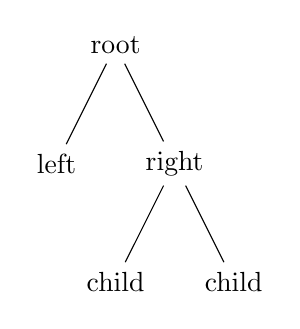
\begin{tikzpicture} % will be written to 'main-figure0.pdf'
  \node {root}
    child {node {left}}
    child {node {right}
      child {node {child}}
      child {node {child}}
    };
\end{tikzpicture}

{
  \tikzset{external/figure name={subset_}}
  A simple image is \tikz \fill (0,0) circle(5pt);. % will be written to 'subset_0.pdf'

  
\begin{tikzpicture} % will be written to 'subset_1.pdf'
     \draw[help lines] (0,0) grid (5,5);
  \end{tikzpicture}
}% here, the old file name will be restored:

\begin{tikzpicture} % will be written to 'main-figure1.pdf'
   \draw (0,0) -- (5,5);
\end{tikzpicture}
\end{document}
\end{codeexample}
	The scope of |figure name| ends with the next closing brace (as all values set by |\tikzset| do).

	Remark: Use |\tikzset{external/figure name/.add={prefix_}{_suffix_}}| to add a |prefix_| and a |_suffix_| to the actual value of |figure name|.
\end{key}


\subsubsection{Remaking Figures or Skipping Figures}
\begin{key}{/tikz/external/force remake=\marg{boolean} (default true)}
	A boolean which is used by |mode=convert with system call|. Every up-to-date check will fail, resulting in automatic regeneration of every figure.

\begin{codeexample}[code only]
\tikzset{external/force remake}

\begin{tikzpicture}
	\draw (0,0) circle(5pt);
\end{tikzpicture}
\end{codeexample}
	You can also use |force remake| inside of a local \TeX\ group to remake only selected pictures. The example
\begin{codeexample}[code only]
\tikz \draw (0,0) -- (1,1);

{
\tikzset{external/force remake}

\begin{tikzpicture}
   \draw (0,0) circle(5pt);
\end{tikzpicture}
}

\tikz \draw (0,0) -- (1,1);
\end{codeexample}
	will only apply |force remake| to the second figure.
\end{key}

\begin{key}{/tikz/external/remake next=\marg{boolean} (default true)}
	A variant of |force remake| which applies only to the next image.
\end{key}

\begin{key}{/tikz/external/export next=\marg{boolean} (default true)}
	A boolean which can be used to disable the export mechanism for single pictures.
\end{key}

\begin{key}{/tikz/external/export=\marg{boolean} (initially true)}
	A boolean which can be used to disable the export mechanism for all pictures inside of the current \TeX-scope. 

\begin{codeexample}[code only]
\begin{document}
\begin{tikzpicture} % will be exported
	...
\end{tikzpicture}

{
\tikzset{external/export=false}
\begin{tikzpicture} % won't be exported
	...
\end{tikzpicture}
...
} 

\begin{tikzpicture} % will be exported
	...
\end{tikzpicture}
\end{document}
\end{codeexample}
	For \LaTeX, the feature lasts until the next |\end|\marg{$\cdot$} (this holds for every call to |\tikzset|).
\end{key}



\subsubsection{Customizing the Externalization}
\begin{key}{/tikz/external/figure list=\marg{boolean} (initially true)}
	A boolean which configures whether a figure list shall be generated. A figure list is an output file named \marg{jobname}|.figlist| which is filled with file names of each figure, one per line.

	This file is not used by \TeX\ anymore, its purpose is to issue the required conversion commands |pdflatex -jobname |\marg{picture file name} \marg{main file} manually (or in a script).

\begin{codeexample}[code only]
\documentclass{article}
% main document, called main.tex
\usepackage{tikz}

\usetikzlibrary{external}
\tikzexternalize[
   mode=graphics if exists,
   figure list=true,
   prefix=figures/]{main} % provide the file's real name

\begin{document}

\tikzsetnextfilename{trees}
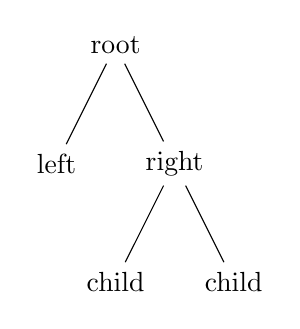
\begin{tikzpicture}
  \node {root}
    child {node {left}}
    child {node {right}
      child {node {child}}
      child {node {child}}
    };
\end{tikzpicture}

\tikzsetnextfilename{simple}
A simple image is \tikz \fill (0,0) circle(5pt);.


\begin{tikzpicture}
   \draw[help lines] (0,0) grid (5,5);
\end{tikzpicture}
\end{document}
\end{codeexample}

\begin{codeexample}[code only]
pdflatex main
\end{codeexample}
generates |main.figlist| containing
\begin{codeexample}[code only]
figures/trees
figures/simple
figures/main-figure0
\end{codeexample}
\end{key}

\begin{key}{/tikz/external/mode=\marg{choice} (initially convert with system call)}
	Configures what to do with \tikzname\ pictures (unless we are currently externalising one particular image, in that case, these modes are ignored).
	
	The choice |only graphics| always tries to replace pictures with external graphics. It is an error if the graphics file does not exist.

	The choice |no graphics| (or, equivalently, |only pictures|) typesets \tikzname\ pictures without checking for external graphics.

	A mixture is |graphics if exists|, it checks whether a suitable graphics file exists and includes it if that is the case. If it does not exist, the picture is typeset using \TeX.

	Mode |list only| skips every \tikzname\ picture; it only generates the file \marg{main file}|.figlist| containing file names for every picture, the contents of any picture environment is thrown away and a replacement text is shown. This implies |figure list=true|.

	The preconfigured mode |convert with system call| checks whether external graphics file are up-to-date and includes them if that is the case. Any picture which is not up-to-date will be generated automatically using a system call. The system call can be configured using the |system call| template. The up-to-date check is simple: if the file does not exist, it is not up-to-date. Furthermore, if one of the |force remake| or |remake next| keys is true, the figure is not up-to-date. In all other case, the file is considered to be up-to-date. Setting this mode automatically disables |figure list| because such a file is not required. If you still need it, you can enable it after setting |mode|.

	Please note that system calls may be disabled for security reasons. For pdflatex, they can be enabled using
\begin{codeexample}[code only]
pdflatex -shell-escape
\end{codeexample}
	while other \TeX\ variants may need other switches. The feature is sometimes called |\write18|.

	A further, rather special mode allows to generate a makefile on-the-fly: |list and makefile| is similar to |list only|: it generates the same file \marg{main file}|.figlist|, but any images which exist already are included as graphics instead of ignoring them. Furthermore, this mode generates an additional file: \marg{main file}.makefile. The work flow idea here is to use
\begin{codeexample}[code only]
% step 1: generate main.makefile:
pdflatex main
% step 2: generate ALL graphics on 2 processors:
make -j 2 main.makefile
% step 3: include the graphics:
pdflatex main
\end{codeexample}
	\noindent This mode is for specialists who like to work with |make|. It allows parallel externalisation of graphics on multi-core systems.
\end{key}


\begin{key}{/tikz/external/verbose IO=\marg{boolean} (initially true)}
	A boolean which configures whether I/O operations shall be listed in the logfile.
\end{key}
\begin{key}{/tikz/external/verbose optimize=\marg{boolean} (initially true)}
	A boolean which configures whether optimization operations shall be listed in the logfile.
\end{key}

\begin{key}{/tikz/external/optimize=\marg{boolean} (initially true)}
	Configures whether the conversion process shall be optimized. This affects only the case when |\jobname| differs from the main file name, i.e. when single pictures are converted.

	In that case, the main file is compiled as usual - but everything except the selected picture is thrown away. If optimization is enabled, all other pictures won't be processed at all. Furthermore, expensive commands which do not contribute to the selected picture will be thrown away as well.

	The default implementation discards |\includegraphics| commands which are \emph{not} inside of the selected picture to reduce conversion time.

	It is possible to add commands which shall be optimized away, see below.
\end{key}

\begin{key}{/tikz/external/optimize command away=\meta{\textbackslash command}\marg{required argument count}}
	Installs commands to optimize \meta{\textbackslash command} away. As is described above, optimization applies to the case when single pictures are converted: one usually doesn't need to process (probably expensive) commands which do not contribute to the selected picture.

	The argument \marg{required argument count} is either empty or a non-negativ integer between $0$ and $9$. It denotes the number of arguments which should be consumed after \meta{\textbackslash command}. In any case, one argument in square brackets after the command will be recognised as well. To be more precise, the following cases for arguments of \meta{\textbackslash command} are supported:
	\begin{enumerate}
		\item If \marg{required argument count} is empty (the default), \meta{\textbackslash command} may take one optional argument in square brackets and one in curly braces (which is also optional).
		\item If \marg{required argument count} is not empty, \marg{\textbackslash command} may take one optional argument in square brackets. Furthermore, it expects exactly \marg{required argument count} following arguments.
	\end{enumerate}

	Example:
\begin{codeexample}[code only]
\tikzset{external/optimize command away=\includegraphics}
\end{codeexample}

\begin{codeexample}[code only]
\newcommand{\myExpensiveMacro}[1]{Very expensive!}

\tikzset{external/optimize command away=\myExpensiveMacro}
\end{codeexample}

\begin{codeexample}[code only]
\newcommand{\myExpensiveMacroWithThreeArgs}[3]{Very expensive!}

\tikzset{external/optimize command away={\myExpensiveMacroWithThreeArgs}{3}}
\end{codeexample}
\begin{codeexample}[code only]
% A command with optional argument:
\newcommand{\aFurtherExample}[3][]{Very expensive!}

% consume only two arguments: the first optional one will be processed
% anyway:
\tikzset{external/optimize command away={\myExpensiveMacroWithThreeArgs}{2}}
\end{codeexample}
	The argument \meta{\textbackslash command} must be the name of a single macro. Any occurance of this macro, together with its arguments, will be removed.
\begin{codeexample}[code only]
\begin{tikzpicture}
	% this picture is currently converted!
\end{tikzpicture}

This here is outside of the converted picture and contains \myExpensiveMacro. It will be discarded.

This call: \myExpensiveMacro[argument=value]{Argument} as well. 
And this here: \myExpensiveMacro{Argument} also.
\end{codeexample}

	The default is to optimize |\includegraphics| away.

	This key is actually a style which sets the |optimize/install| and |optimize/restore| keys.
\end{key}

\begin{key}{/tikz/external/optimize/install}
	A command key which contains code to install optimizations. You can append code here (or clear the macro) if you need to modify the optimization.
\end{key}
\begin{key}{/tikz/external/optimize/restore}
	A command key which contains code to undo optimizations. You can append code here (or clear the macro) if you need to modify the optimization.
\end{key}

\begin{key}{/tikz/external/only named=\marg{boolean} (initially false)}
	If enabled, only pictures for which file names have been set explicitly using |\tikzsetnextfilename| will be considered, no file names will be generated automatically.
\end{key}

\begin{key}{/pgf/images/include external (initially \textbackslash pgfimage\{\#1\})}
\index{External Graphics!Bounding Box Issues}
	This key constitutes the public interface to exchange the |\includegraphics| command used for the image inclusion.

	Its description can be found in the corresponding basic layer documentation on page~\pageref{pgf:includeexternalkey}.

	Just one example here: you can use
\begin{codeexample}[code only]
\pgfkeys{/pgf/images/include external/.code={\includegraphics[viewport=0 0 211.28 175.686]{#1}}}
\end{codeexample}
	to manually change the viewport (bounding box) for included graphics.
	
	If you want to limit the effects of this key to just one externalized figure, use
\begin{codeexample}[code only]
{
\pgfkeys{/pgf/images/include external/.code={\includegraphics[viewport=0 0 211.28 175.686]{#1}}}
\begin{tikzpicture}
	...
\end{tikzpicture}
}% this brace ends the effect of `include external'
\end{codeexample}
\end{key}

\subsection{Using external graphics without \textmd{\pgfname}\ installed}
\label{section-libs-external-nopgf}
Given that every picture has been exported correctly, one may want to compile a file without \pgfname\ and \tikzname\ installed. \tikzname\ comes with a minimal package which contains just enough commands to replace every |tikzpicture| environment and the |\tikz| short command with the appropriate external graphics. It can be found at
\begin{codeexample}[code only]
latex/pgf/utilities/tikzexternal.sty
\end{codeexample}
\noindent and needs to be used instead of |\usepackage{tikz}|. Our example from the beginning thus becomes
\begin{codeexample}[code only]
\documentclass{article}
% main document, called main.tex
%\usepackage{tikz}

\usepackage{graphicx}
\usepackage{tikzexternal}

%\usetikzlibrary{external}
\tikzexternalize{main} % provide the file's real name

\begin{document}
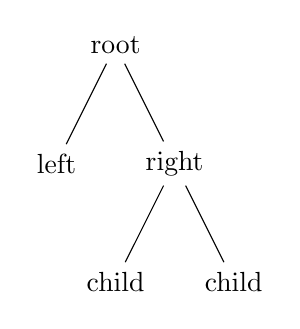
\begin{tikzpicture}
  \node {root}
    child {node {left}}
    child {node {right}
      child {node {child}}
      child {node {child}}
    };
\end{tikzpicture}

A simple image is \tikz \fill (0,0) circle(5pt);.
\end{document}
\end{codeexample}
\noindent where the following files are necessary to compile the document:
\begin{codeexample}[code only]
tikzexternal.sty
main.tex
figures/main-figure0.pdf
figures/main-figure1.pdf
figures/main-figure2.pdf
\end{codeexample}
\noindent If there are any `|.dpth|' files, for example |figures/main-figure0.dpth|, these files are also required. They contain information for the \tikzname\ |baseline| option.

Just copy the |.sty| file into the directory of your |main.tex| file and use it as part of your document.

Please keep in mind, that only |tikzpicture| environments and |\tikz| short images are available within the externalization framework. Additionally, calls to |\tikzset| and |\pgfkeys| won't lead to compilation errors because they are simply ignored. But since |pgfkeys| is not available, any option supplied to |\tikzexternalize| is \emph{ignored}.

Please use |\tikzsetexternalprefix| instead of the |prefix| option.

\subsection{Externalization and bounding box restrictions}
Bounding box restrictions provide no problem when used with \eps\ graphics (see the next section). However, they pose problems for |pdflatex|, so you may need to use the |latex| / |dvips| combination if you use bounding box restrictions and externalization.

\subsection{\eps\ Graphics}
It is also possible to use \eps\ graphics instead of \pdf\ files. There are different ways to produce them, for example to use |pdflatex| and call |pdftops -eps |\marg{pdf file} \marg{eps file} afterwards. You could add this command to the |system call| option.

Alternatively, you can use |latex| and |dvips| for image conversion as is explained for the |system call| option, see page~\pageref{extlib:systemcall:option}. See the documentation for the basic level externalization in section~\ref{section-external} for restrictions of other drivers.

\subsection{Interoperability with the basic layer externalization}
This library is fully compatible with |\beginpgfgraphicnamed|$\dotsc$|\endpgfgraphicnamed| environments. However, you will need to use the |export next=false| key to avoid conflicts:
\begin{codeexample}[code only]
\beginpgfgraphicnamed{picture4}
\tikzset{external/export next=false}
\begin{tikzpicture}
   \draw (0,0) -- (4,4);
\end{tikzpicture}
\endpgfgraphicnamed
\end{codeexample}
Please keep in mind that file prefixes do not apply to the basic layer.
